% Created 2024-10-16 śro 21:35
% Intended LaTeX compiler: pdflatex
\documentclass[../main.tex]{subfiles}

% \usepackage[a4paper, margin=3cm]{geometry}
% \usepackage{amssymb} // not working

\usepackage[T1]{fontenc}
\usepackage[utf8]{inputenc}
\usepackage{graphicx}
\usepackage{longtable}
\usepackage{wrapfig}
\usepackage{rotating}
\usepackage[normalem]{ulem}
\usepackage{amsmath}
\usepackage{capt-of}
\usepackage{hyperref}
\usepackage{siunitx}
\usepackage{float}
\usepackage[polish]{babel}

\graphicspath{{../}}
\author{Wojciech Paderewski}
\date{\today}
\title{Schemat projektu}
\hypersetup{
 pdfauthor={Wojciech Paderewski},
 pdftitle={Schemat projektu},
 pdfkeywords={},
 pdfsubject={},
 pdflang={Polish}}

\begin{document}
Szczegółowa koncepcja układu została podzielenia na poszczególne sekcje układu.

\subsubsection{Sterowanie lampami nixie}
Kluczowym jest wybór sterownia lampami nixie, ponieważ na podstawie tego wyboru zostanie zaprojektowany pozostała cześć układu.
Zgodnie z analizą przeprowadzoną w podrozdziale \ref{sec:sterownie_lampi}, zdecydowano się na sterowanie lampami za pomocą rejestrów przesuwnych wysokiego napięcia.
Zastosowanie tego rozwiązania pozwala na zredukowanie ilości potrzebnych wyprowadzeń mikrokontrolera do sterowania lampami. Ten typ sterowania jest łatwy w implementacji,
wymaga jedynie wgrania odpowiednich danych do rejestrów przesuwnych, a następnie zatrzaśnięcie
 wyjścia, co pozwala na wyświetlenie odpowiedniej cyfry na lampie.

Niezależnie od wyboru lamp każda ma 10 katod z cyframi i jedną katode od kropki dziesiętnej, więc wymagane jest 11 wyjść na każdą lampę.
Dostępne w sprzedaży są rejestry 32 bitowe, co pozwala na sterowanie 3 lampami nixie bez kropek i jedną neonówką która będzie
służyć jako separator między godzinami a minutami oraz między minutami a sekundami. Do sterownia kropkami dziesiętnymi zostaną użyte tranzystory wysokiego napięcia podłączone do wyjść mikrokontrolera,
ponieważ nie opłacalnym jest dodawanie kolejnego rejestru przesuwnego wysokiego napięcia tylko do sterowania kropkami dziesiętnymi.

Wynika z tego, że potrzebne są 2 rejestry przesuwne wysokiego napięcia do sterownia lampi i neonówkami oraz 6 tranzystorów wysokiego napięcia do sterowania kropkami dziesiętnymi.
Do sterowania rejestrami prawdopodobnie będzie potrzebny konwerter poziomów logicznych, ponieważ mikrokontroler ESP32-S3 zasilany jest napięciem \SI{3.3}{\volt}, a rejestry prawdopodobnie będą operować na wyższym napięciu.
\subsubsection{Mikrokontroler}
Wybór sposobu sterowania lampami nixie wpłynął na wybór mikrokontrolera, ponieważ musi on posiadać odpowiednią ilość pinów GPIO oraz musi być w stanie generować sygnał zegarowy.
Potrzebne jest 9 pinów GPIO do pełnego sterownia lampami oraz kropkami dziesiętnym, do tego trzeba pamiętać o zapasie pinów na pozostałe funkcje. W zwiazku z tym
wybrano mikrokontroler ESP32-S3, który posiada 45 programowalnych GPIO, co pozwala na swobodne zaprojektowanie reszty układu. Ma też on dużą zaletę w postaci kontrolera USB/JTAG,
dzięki czemu nie jest potrzebny dodatkowy programator do programowania układu. Jest to też popularny mikrokontroler dla którego istnieje dużo bibliotek i przykładów.

\subsubsection{Źródło dźwięku}
Jako źródło dźwięku wybrano głośnik piezoelektryczny, który jest prostym elementem i nie wymaga dodatkowego wzmacniacza. Jego zaletami są niski pobór prądu, małe rozmiary i niska cena.
Sterowanie odbywa się za pomocą sygnału PWM, który pozwala generować proste melodie. Głośnik piezoelektryczny jest wystarczająco głośny
aby być słyszalnym w pomieszczeniu, w którym będzie znajdował się budzik.

\subsubsection{Pasek LED}
Pasek LED będzie służył jako dodatkowe źródło światła, które będzie sygnalizować alarm i jako element estetyczny. Pasek ten musi 
zawierać w sobie adresowane diody LED, które pozwolą na wyświetlanie różnych kolorów (RGB).
Rozwiązanie to jest proste w implementacji, wystarczy podłączyć go do pinu GPIO mikrokontrolera i za pomocą sygnału PWM można sterować jasnością.

\subsubsection{Interfejs użytkownika}
Interfejs użytkownika będzie składał się z enkodera z przyciskiem, który będzie służył do regulacji jasności, a przycisk do wyłączania alarmu.
Enkoder jest też na tyle uniwersalnym rozwiązaniem, które pozwala na mnogość kombinacji sterowania, ale wygodniejsze jest korzystanie z aplikacji mobilnej.

\subsubsection{Zasilanie}
Kluczowe jest zaprojektowanie przetwornicy wysokiego napięcia do zasilania lamp nixie, ponieważ jest to najbardziej wymagający element układu.

Możliwe są dwa rozwiązania:
\begin{itemize}
    \item Przetwornica typu flyback
    \item Przetwornica typu boost
\end{itemize}

Przetwornica typu flyback ma zaletę w postaci izolacji galwanicznej między wejściem a wyjściem oraz jest możliwe zaprojektowanie przetwornicy z napięciem zasilania \SI{5}{\volt}. 
Wadą jest to, że jest potrzebny transformator który jest drogi i trudno dostępny, do tego jest to bardziej skomplikowane rozwiązanie na etapie projektowania.

Ze względu na duży problem ze znalezieniem transformatora, zdecydowano się na przetwornicę typu boost, która jest prostsza w implementacji i tańsza. 
Wadą jest to, że nie ma izolacji galwanicznej między wejściem a wyjściem, ale w tym przypadku nie jest to wymagane.
Następnym krokiem było wybranie jednej z dwóch konfiguracji układu:

\begin{itemize}
    \item USB-C jako zasilanie zewnętrzne, przetwornica typu boost z zasilacza \SI{5}{\volt} na \SI{12}{\volt} i przetwornica typu boost z zasilacza \SI{12}{\volt} na wysokie napięcie
    \item Złącze DC jako zasilanie zewnętrzne, przetwornica typu boost z zasilacza \SI{12}{\volt} na wysokie napięcie oraz przetwornica typu buck z zasilacza \SI{12}{\volt} na \SI{5}{\volt}
\end{itemize}

Wadą pierwszej konfiguracji jest to, że niemożliwym będzie jednoczesne programowanie i zasilanie układu, ponieważ złącze USB-C podłączone do komputera ma niską wydajność prądową.
Dla USB 2.0 wynosi ona 500mA, a dla USB 3.0 wynosi 900mA, co jest niewystarczające dla zasilania układu. Brak możliwości jednoczesnego zasilania i programowania było by 
dużym problemem na etapie pisania oprogramowania, więc zdecydowano się na drugą konfigurację.

Wybrano więc przetwornicę typu boost, która będzie zasilana z zasilacza \SI{12}{\volt}, a wyjście będzie podłączone do anod lamp nixie.
Do tego będzie potrzebne zasilanie \SI{5}{\volt} dla paska LED oraz \SI{3.3}{\volt} dla mikrokontrolera. Moduł zasilania \SI{5}{\volt} będzie zasilał pasek LED, który potrafi pobrać większy prąd,
to ze względu na zachowanie wysokiej efektywności, zdecydowano się na przetwornicę typu buck. Moduł zasilania \SI{3.3}{\volt} będzie zasilaniem mikrokontrolera, więc wystarczy zastosować
stabilizator liniowy.

Można, więc podzielić zasilanie na 3 pod moduły:
\begin{itemize}
    \item Przetwornica typu boost z zasilacza \SI{12}{\volt} na wysokie napięcie
    \item Przetwornica typu buck z zasilacza \SI{12}{\volt} na \SI{5}{\volt}
    \item Stabilizator liniowy z zasilacza \SI{5}{\volt} na \SI{3.3}{\volt}
\end{itemize}

Wynika z tego, że urządzenie będzie posiadać 3 złącza:
\begin{itemize}
    \item Złącze USB-C do programowania mikrokontrolera
    \item Złącze DC do zasilania układu
    \item Złącze typu goldpin jako złącze do komunikacji szeregowej wykorzystywane w procesie uruchamiania układu
\end{itemize}

\subsubsection{Szczegółowy schemat projektu}
\begin{figure}[H]
    \centering
    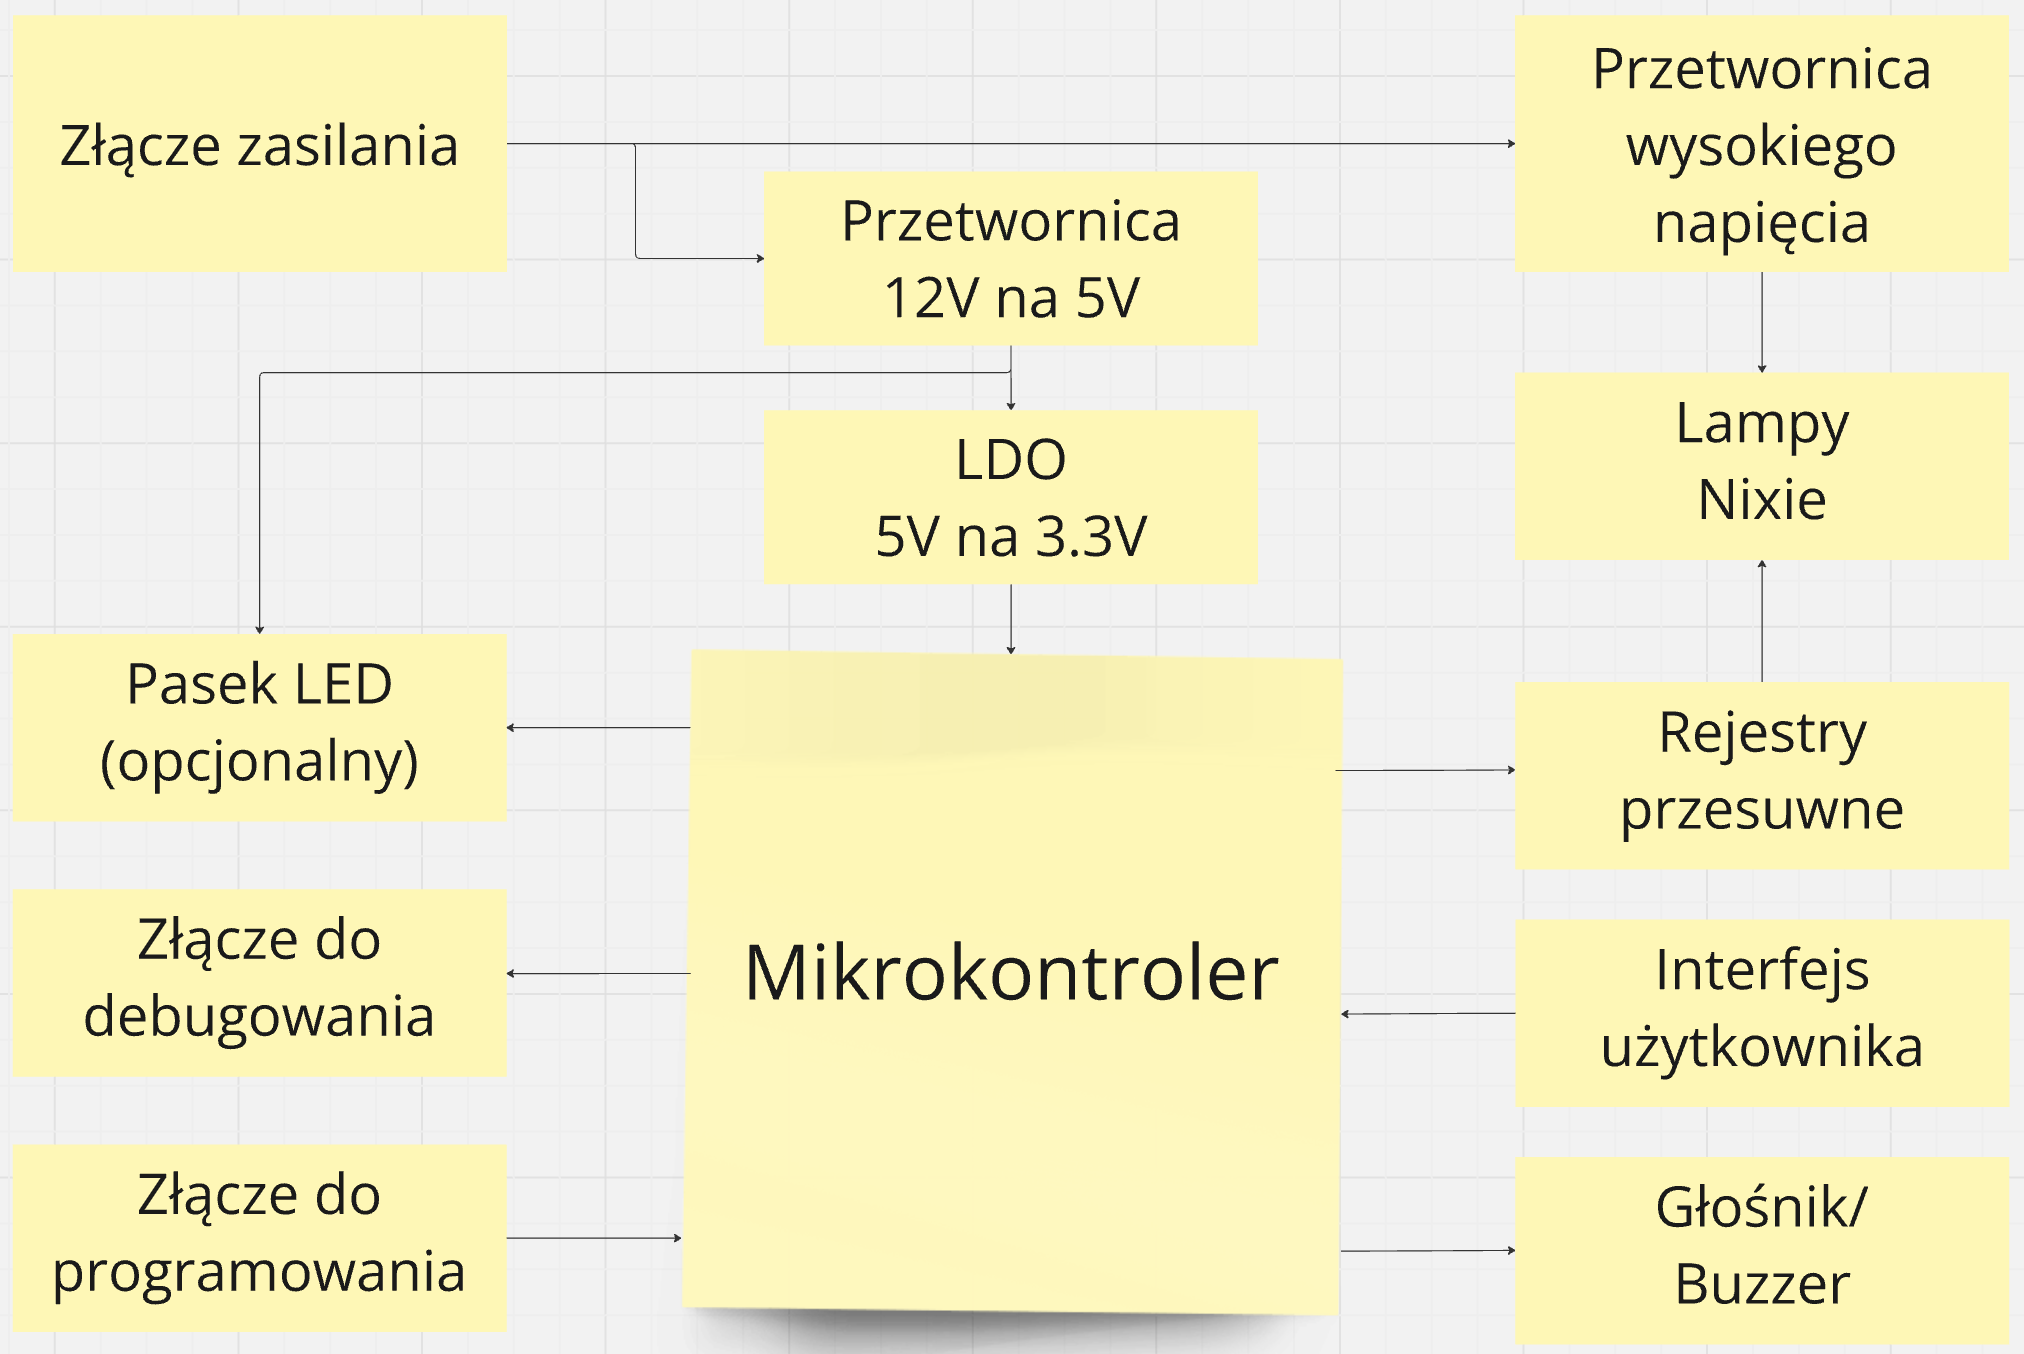
\includegraphics[width=1\textwidth]{schemat_szcz.png}
    \caption{Schemat blokowy projektu}
    \label{fig:schemat_projektu}
\end{figure}

\end{document}
